\label{Section:experiments}
\subsection{Infrastructure overviews}
Caliburn
Caliburn is the new supercomputer from RDI2, which is ranked \#166 worldwide in the Top500 list of June 2016. This system is based on TatTwin SuperServer solution and it has 560 nodes containing 20,160 cores, 140 TB of RAM memory, 218 TB of non-volatile memory and 100 Gbps Omni-Path fabric (OPA) interconnection, which deliver performance of 603 TFLOPS with a peak performance of 677 TFLOPS.  Other details of each node?s hardware is given in Table \ref{table:caliburn_hardware_specification}.

\begin{table}[H]
\begin{center}
\begin{tabular}{|l|l|}
	\hline
	\textbf{H/W Type} & \textbf{H/W Detail}\\ \hline
    CPU & 2\* Intel Xeon E5-2695v4\\ 		
    \hline
    CPU frequency & 2.1 GHz\\
    \hline
    \# of Cores & 2\* 18\\
    \hline
    Cache & 2\* 45 MB\\
    \hline
    Memory &\\
    \hline
    Disk & \\
    \hline
    Network bandwidth & \\
    \hline
\end{tabular}
\caption{Caliburn hardware specification}
\label{table:caliburn_hardware_specification}
\end{center}
\end{table}



\subsection{Power measurement}
\subsubsection{RAPL}
From Intel Sandy Bridge family, Intel released Power Gadget API using RAPL to provide power measurements for components within CPU, including current estimated processor power, current processor frequency, base frequency, thermal design power (TDP), current temperature, timestamps and etc. We use it to collect the processor?s current estimated power consumption (package power). RAPL measuring power data through reading Machine-Specific Registers (MSRs) which frequency can up to 1 KHz. But to reduce the interference, we set the measuring ratio to 1 Hz. According to [in-situ paper], the overhead of setting RAPL at 1 Hz frequency is increase 0.2 W in average, which is negligible. 

\subsubsection{SMCIPMITOOL}
The Caliburn supports Intelligent Platform Management Interface (IPMI), which is a set of computer interface specifications that is led by Intel. [wiki  https://en.wikipedia.org/wiki/Intelligent\_Platform\_Management\_Interface] This IPMI allow administrators to manage the system remotely and monitor platform status as well, such as system power supplies, temperatures, fans and ,etc. The Caliburn vendor Supermicro provides a tool SMCIPMITOOL that allows users to interface with IPMI devices via a command line interface.[ftp://ftp.supermicro.com/utility/SMCIPMItool/SMCIPMITool\_User\_Guide.pdf] In the current system set up, the SMCIPMITOOL can provide us system-wider total power measurement of four nodes at frequency of 0.25Hz, one time per four seconds. Due to the limitation of wide nodes? measuring range and relatively low sampling ratio, we will launch our application from the start node, execute relatively long time and repeat the experiment to eliminate extreme value.



\subsection{Performance measurement}
To quantify the scientific impact of our proposed strategy, in addition to measuring power data, we also using two profiling tools to measure the I/P, memory, networking and CPU utilization. Perf is is a profiler tool for Linux, it offers a rich set of commands to collect and analyze performance and trace data. We use ?perf stat? to gather system performance counter statistics, such as number of instructions, CPU cycles, cache-misses and, etc. In the meantime, we also utilize Linux command Sar (System Activity Report), which can report on various system loads, to measure memory/paging, device load and network.



\subsection{Application configurations}
These four simulation applications are simulating different problems, but they all based on AMR algorithm, which uses a hierarchical grid structure, and fill finer patches on the region of interest. We tune their refinement level via their input configuration, to have high, medium and low resolutions.


\subsection{Methodology}
\subsubsection{Finding appropriate power value, using power cap}
In the previous section, we conclude that the application execution time will decrease as level of refinement/resolution decrease or increase as capping down CPU power. In order to keep application execution time the same with high, medium and low resolution, we first record the execution time of high resolution without implement power cap, and then iteratively capping down CPU power by 10 W for running application in medium or low resolution, until their execution time is matching the high resolution?s execution time within 5\% difference. In this way, we can get the appropriate power cap value for each level of resolution.

\subsubsection{Measuring performance}
This experiment is running on 512 cores across 15 nodes. However, due to the limitation of Perf and Sar, they only can profile a single node. Therefore, we only profile the node that launch the experiment. For example, the experiment is running from node 1 to node 15, then we only measure the performance of node 1. In addition, the power consumption measurement covers all the 15 nodes. SMCIPMITOOL is running on login node, and can measure every node?s power consumption.


**************************Below is the old contents*************************
\subsubsection{Power measurement methodology}
Our experiment platform CAPER is instrumented with both coarse- and fine-grained power metering at server level. On the one hand, an instrumented Raritan iPDU PX2-4527X2U-K2 provides power measurements at 1 Hz. While, on the other hand, a Yokogawa DL850E ScopeCorder provides voltage and current measurement for all nodes through 1 Ms/s modules, and can sample power data at rate of up to 10 KHz. In addition to those server level measurement, we have RAPL meter to provide power measurement at a up to 20Hz sampling rate in processor level. 


\textbf{Use of RAPL power metering}\\
RAPL meter measuring power through reading Machine-Specific Registers (MSRs). Intel released Power Gadget API for using RAPL. This API is a framework that provides very comprehensive information including reading current estimated processor power, current processor frequency, base frequency, thermal design power (TDP), current temperature, timestamps and etc. Also, Intel gives a ready-to-use software-based power monitoring tool called Intel Power Gadget, this has a completed interface for using RAPL. We are using this to measure the processors power usage. 


\textbf{RAPL meter sampling frequency considerations}\\
Thought, according to Intel’s manual,\cite{intel64and} RAPL MSRs would update at rate of once every 1 ms, using very lower frequency (e.g. less than 20 ms) may result in significant overhead and might also increase the power consumption, which would make the data less meaningful.\cite{usingtheintelpowergadgetapionmacosx} Also, since the instantaneous processor frequency would change very frequently, sampling data may be more useful if you sample often and average the samples overtime. So, Intel recommend sampling frequency of 50 ms or upper. For our experiment, we don’t require high resolution power data, so we choose to sample twice per second.


\textbf{Reading power measurement data from PDU}\\
Raritan PDU keep measuring the whole servers power consumption and writing the power measurement data to power log files with timestamp. CAPER has eight nodes, so we extract real-time power measurement data and the timestamp from each node’s power log file after simulation started using Simple Network Management Protocol (SNMP) queries to the PDU from a side script running in an independent node.


\subsubsection{AMR resolution adjustment}
LMC simulation program is based on AMR algorithm, which uses a hierarchical grid structure, and fill finer patches on the region of interest. Therefore, the simulation’s resolution from the computational point of view is mainly directed from the AMR algorithm resolution configuration. There are many parameters controlling AMR solution, but in the work, only those four parameters listed in Table \ref{table:table_tune_resolution} have been used to tune the simulation resolution. 


\begin{table}[H]
\begin{center}
\begin{tabular}{|l|l|}
	\hline
	\textbf{Parameter} & \textbf{Definition}\\ \hline
    amr.n\_cell & Number of cells in each direction at the coareset level\\ 		\hline
    amr.max\_level & Number of levels of refinement above the coarsest level\\
	\hline
    amr.ref\_ratio & Ratio of coarse to fine grid spacing between subsequent levels\\
    \hline
    amr.regrid\_int & How often to regrid\\
    \hline
\end{tabular}
\caption{AMR parameters which are used to tune simulation resolution}
\label{table:table_tune_resolution}
\end{center}
\end{table}

Each parameter has different impact on the resolution, which is illustrated with the example use case shown in Figure \ref{fig:AMR_resolution_explaination}. The parameters of the example case are discussed as follows.

Example case:
\begin{itemize}
\item amr.n\_cell = 32 32 32
\end{itemize}
This would define the domain size (at coarsest level) to have 32 cells in the x-direction, 32 cells in the y-direction and 32 cells in the z-direction. (If it is in the 2D input file, the last number will be ignored). As shown in Figure \ref{fig:AMR_resolution_explaination}, there are 32 cells in both x and y direction.

\begin{itemize}
\item amr.max\_level = 2
\end{itemize}
This would set a maximum of 2 refinement levels in addition to the coarse level. Within the calculation, the number of refinement level must be $\leqslant$ amr.max\_level, but it can be change in time and it is not necessary always be equal to amr.max\_level. Because these additional levels will only be created if the tagging criteria are such that cells are flagged as needing refinement. Figure \ref{fig:AMR_resolution_explaination} shows the mesh grids with maximum of 2 refinement levels.

\begin{itemize}
\item amr.ref\_ratio = 4 2
\end{itemize}
Refinement ration means how many individual cells will a cell be divided into. For example in the left-hand side Figure \ref{fig:AMR_resolution_explaination}, Setting amr.ref\_ratio = 4 2 means dividing cell into 4 cells from levels 0 and 1, and dividing cell into 2 from levels 1 and 2.

\begin{itemize}
\item amr.regrid\_int = 2
\end{itemize}
This would tell the code to regrid every 2 steps. This means level l+1 grids will be created every 2 level l time steps.


\begin{figure}[H]
	\centering
    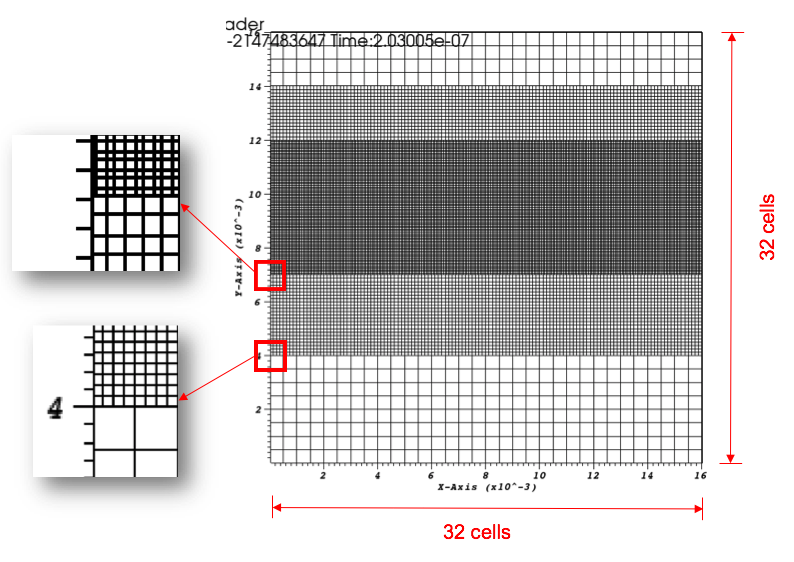
\includegraphics[width=8cm]{figs/AMR_resolution_explaination.png}
        \caption{AMR mesh grids outcome of the example configuration}
        \label{fig:AMR_resolution_explaination}
\end{figure}






